%%%%%%%%%%%%%%%%%%%%%%%%%%%%%%%%%%%%%%%%%%%%%%%%%%%%%%%%%%%%%%%%%%%%%%%%%%%%%%%%%%
\begin{frame}[fragile]\frametitle{}
\begin{center}
{\Large Notes from Shri M's Teachings}
\end{center}
\end{frame}

%%%%%%%%%%%%%%%%%%%%%%%%%%%%%%%%%%%%%%%%%%%%%%%%%%%%%%%%%%%
\begin{frame}[fragile]\frametitle{Kriya Yoga}

	\begin{itemize}
	\item $kriya$ : technique after following rules-regulations
	\item Life energy is dissipating everywhere, say, 108 centers $nadis$
	\item $shwas$ (breath) is linked to $prana$ (life energy)
	\item $kriya$ tries to balance $prana$
	\item Gather your energies in one point, save, avoid wastage. 
	\item You become full of energy/light.
	\item $kriya$ is not a must for spiritual awakening though, e.g. $mirabai$, $ramana-maharshi$.
	\end{itemize}

{\tiny (Ref: Sri M-(Short Video)- ``What is Kriya Yoga?'' - YouTube)}

\end{frame}


%%%%%%%%%%%%%%%%%%%%%%%%%%%%%%%%%%%%%%%%%%%%%%%%%%%%%%%%%%%
\begin{frame}[fragile]\frametitle{Hindu Scriptures}

\begin{center}
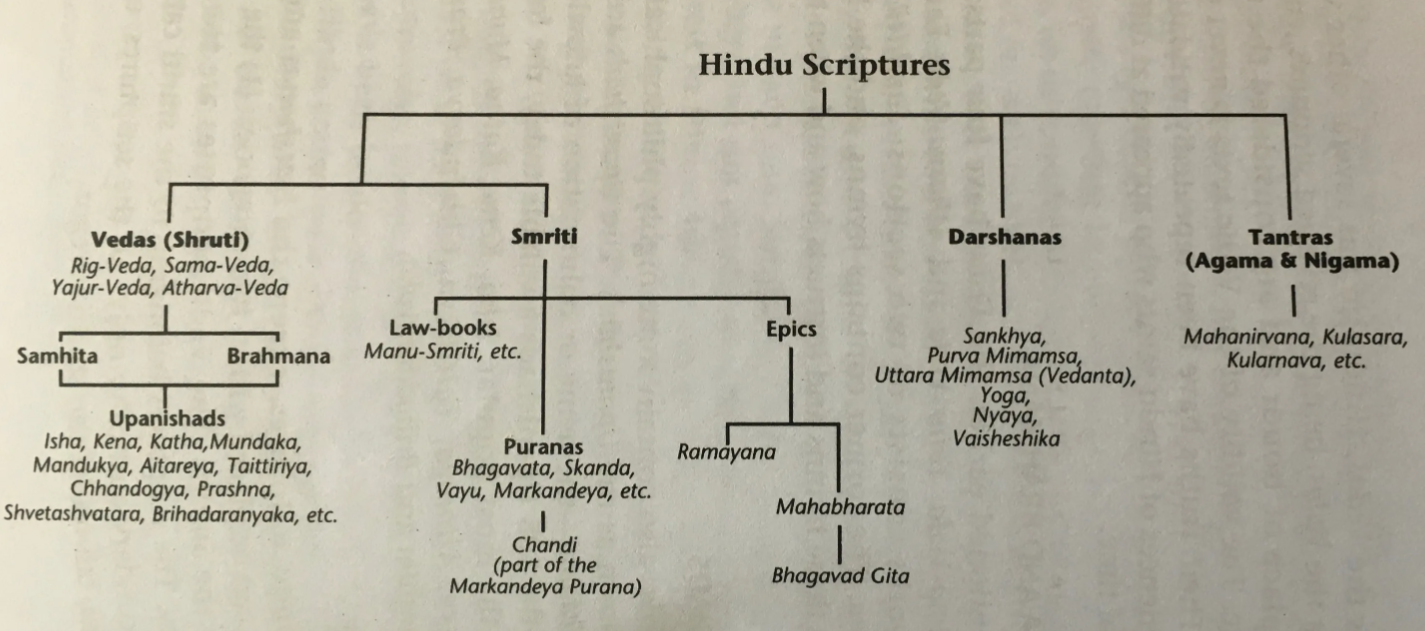
\includegraphics[width=\linewidth,keepaspectratio]{veda1}
\end{center}	 

{\tiny (Ref: Essence of the Upanishads \& An Overview of Hindu Scriptures - vak1969.com)}

\end{frame}

%%%%%%%%%%%%%%%%%%%%%%%%%%%%%%%%%%%%%%%%%%%%%%%%%%%%%%%%%%%
\begin{frame}[fragile]\frametitle{Vedanta in Daily Life}

	\begin{itemize}
	\item All activities are aiming at 'completeness'($purna$)
	\item Veda: brahamana (rituals), samhita (singing), arayanyaka (deep knowledge), Vedanta (upanishads-explains veda)
	\item Leave the cocoon, like a moth becomes a butterfly.
	\item Vedanta in Daily Life: Essenes of god in everyone, so why harm it and also why harm others. Lead meditative life. Read Bhagavat Geeta.
	\end{itemize}

{\tiny (Ref: How to practise Vedanta in daily life | Talk \& Q\&A | Sri M - YouTube)}

\end{frame}

%%%%%%%%%%%%%%%%%%%%%%%%%%%%%%%%%%%%%%%%%%%%%%%%%%%%%%%%%%%
\begin{frame}[fragile]\frametitle{Meditation}

	\begin{itemize}
	\item Even though "om soh", a simple technique, do it with focus. You will get it automatically when you deserve.
	\item You all need not be $sanyasi$, but being in family also you can meditate.
	\item Equanimity ($sthitapradnya$) once reached, can make you eligible to teach
	\item $kaivalya$ ($sankhya$ and $patanjali$) root is $keval$, there is nothing but universal witness, not even me.
	\end{itemize}

{\tiny (Ref: On Meditation | Navbharat Times Intvw | July 2019 Sri M - YouTube)}

\end{frame}
